%!TEX program = xelatex
%!BIB program = bibtex
\documentclass[cn,black,12pt,normal]{elegantnote}
\usepackage{float}
\usepackage{hyperref}
\usepackage{amsmath}
\usepackage{amsfonts}
\usepackage{amssymb}
\usepackage{siunitx}[=v2]
\usepackage{fancyhdr}
\usepackage{newtxtext}
\usepackage{algorithm}
\usepackage{algorithmic}
\newcommand{\uct}[1]{\textsuperscript{\textsuperscript{\cite{#1}}}}
\renewcommand{\tablename}{\textbf{Table}}
\renewcommand{\figurename}{Figure.}
\renewcommand{\refname}{References}
\renewcommand{\contentsname}{Contents}
\renewcommand{\versiontext}{Version: }
\renewcommand{\updatetext}{Update: }
\PassOptionsToPackage{no-math}{fontspec}
\lstset{basicstyle=\footnotesize\ttfamily\color[RGB]{50,0,130},numbers=none,frame=trBL}

\sisetup{mode=text}
\sisetup{range-phrase = \text{ \textasciitilde }}
\pagestyle{fancy}
\fancyhead[L]{School of Software Engineering, Tongji University}
\fancyhead[R]{Data Structure Projects}
\renewcommand{\headrulewidth}{1pt}

\title{Keyword\\关键字检索系统}
\author{1951510\; 姜文渊}
\institute{\small \url{https://github.com/jwyjohn/Jwy_DataStructureHomework}}
\version{0.50}
\date{\today}

\begin{document}

\maketitle

\textbf{Algorithms involved:} Knuth–Morris–Pratt algorithm, Dynamic programming

\tableofcontents

\section{Introduction}
A string is generally defined as a sequence of characters. Files on a computer system can be seen as a string of bits, and under some encoding rules (like  ASCII,EBCDIC or UTF), they can be seen as a string. One of user's needs when working with files is that, they need to know if a string is in a file. If it is in the file, they want to know how many times do they appear and where are they, \textbf{as FAST as possible}.

Therefore, string-searching algorithms, are of much importance. Sometimes they are also called string-matching algorithms, which represents an important class of string algorithms that try to find a place where one or several strings (also called patterns) are found within a larger string or text.\uct{wiki:String-searching_algorithm}

In this project, the author implemented a simple text editor with the string search function. The algorithm behind the search function is the famous Knuth–Morris–Pratt algorithm (aka. KMP algorithm), which makes the search more efficient.

\section{Demostration}

\subsection{Compile and run the program}

On linux platform with \lstinline{make} and a \lstinline{g++} which supports C++ 11 Standard, just \lstinline{cd} to the \lstinline{./linux} and run \lstinline{make build}. The binary executable will be generated in the same dirctory named as \lstinline{a.out} or \lstinline{keyword}, according to the configurations in the \lstinline{Makefile}. Use \lstinline{./a.out} or \lstinline{./keyword} to run the program.

The program is an interactive shell, where you can input commands and get results.

\begin{figure}[H]
    \centering
    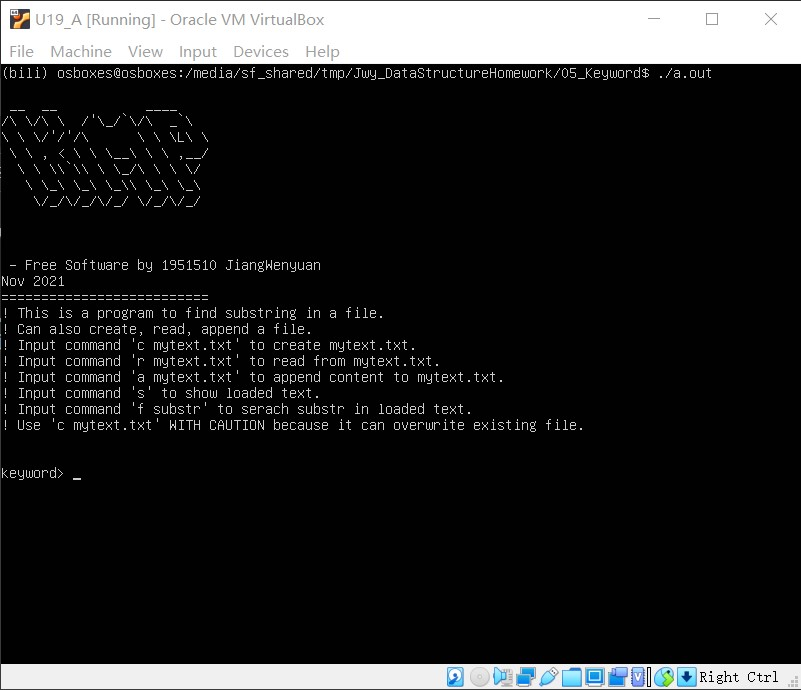
\includegraphics[width=0.6\linewidth]{image/kmp_01.jpg}
    \caption{The user interface of the program}
\end{figure}

Usage of commands can be found on the main screen, and the \lstinline{help} command can give you information about theses commands.  All available commands is listed below.

\begin{enumerate}
    \item \lstinline{help} : Show help for a certain command.
    \item \lstinline{exit} : Exit the program.
    \item \lstinline{c [filename]} : Create a new text file from user input (press Ctrl+D to end input), where \lstinline{[filename]} is the created filename. Pay attention to the filename, for if the file with the same name already exists, it will overwrite the existing file without prompt.
    \item \lstinline{r [filename]} : Read from a textfile, where \lstinline{[filename]} is the filename. The contents of the file is then loaded into memory.
    \item \lstinline{a [filename]} : Append text to a file from user input (press Ctrl+D to end input).
    \item \lstinline{s} : Show the loaded file.
    \item \lstinline{f [string]} : Find the string in loaded file.
\end{enumerate}
Note that if a user inputs invalid commands or arguments, the program will be robust enough (at least to some extent) to detect the exception and return an error message. Detailed Demostration of this feature can be explored when using this program.

\subsection{Create a new file for searching}

Type \lstinline{c test.c} to create \lstinline{test.c} for further operation. We enter the famous Hello World source code to the file and press Ctrl+D to end input.

\begin{figure}[H]
    \centering
    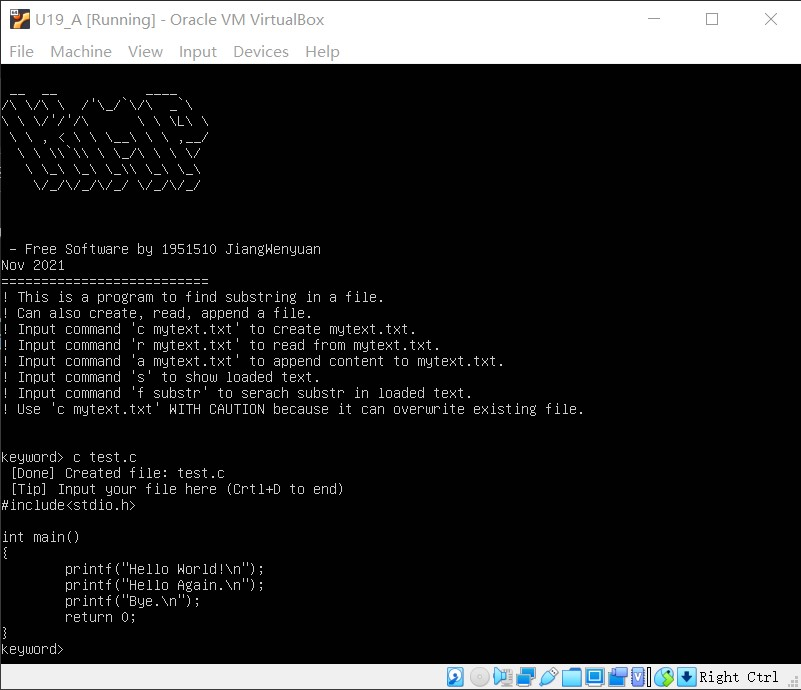
\includegraphics[width=0.6\linewidth]{image/kmp_02.jpg}
    \caption{Use \lstinline{c test.c} to create a new file}
\end{figure}

\subsection{View the created file}
Type \lstinline{r test.c} and then \lstinline{s} to view the file \lstinline{test.c}. If you just created the file, only \lstinline{s} will work.

\begin{figure}[H]
    \centering
    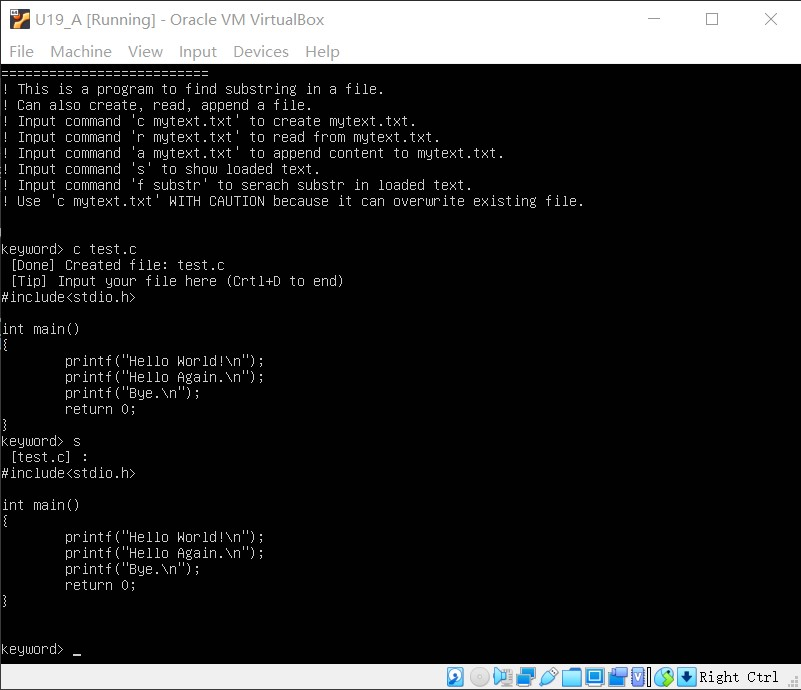
\includegraphics[width=0.6\linewidth]{image/kmp_03.jpg}
    \caption{Use \lstinline{s} to view file}
\end{figure}

\subsection{Search a string}

Type \lstinline{f printf} to search the string \lstinline{printf} in loaded file.

\begin{figure}[H]
    \centering
    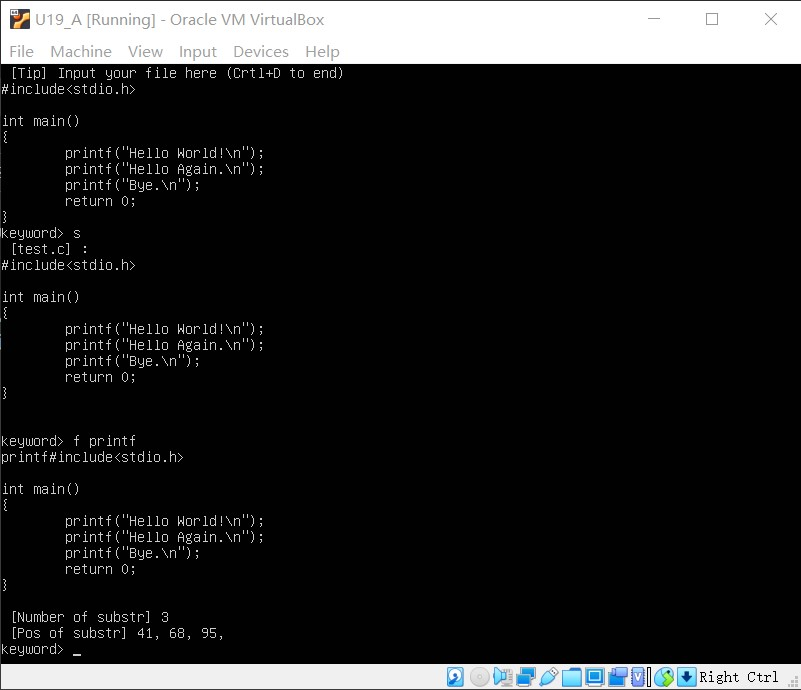
\includegraphics[width=0.6\linewidth]{image/kmp_04.jpg}
    \caption{Use \lstinline{f printf} to search a substring}
\end{figure}

As you can see, the number of substrings and their position is printed.

We load another larger file to memory and search \lstinline{printf}, and the result is shown below.

\begin{figure}[H]
    \centering
    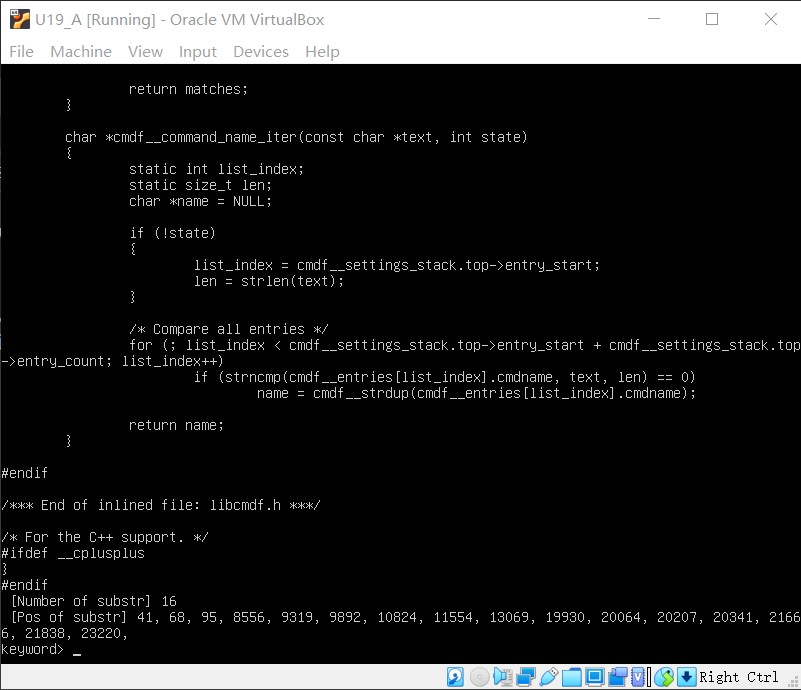
\includegraphics[width=0.6\linewidth]{image/kmp_05.jpg}
    \caption{Use \lstinline{f printf} to search a substring}
\end{figure}

All 16 \lstinline{printf} are found, with their position outputed.

\subsection{Append to a file}
Type \lstinline{a test.c}. We append some comments to the Hello World source code and press Ctrl+D to end input.
\begin{figure}[H]
    \centering
    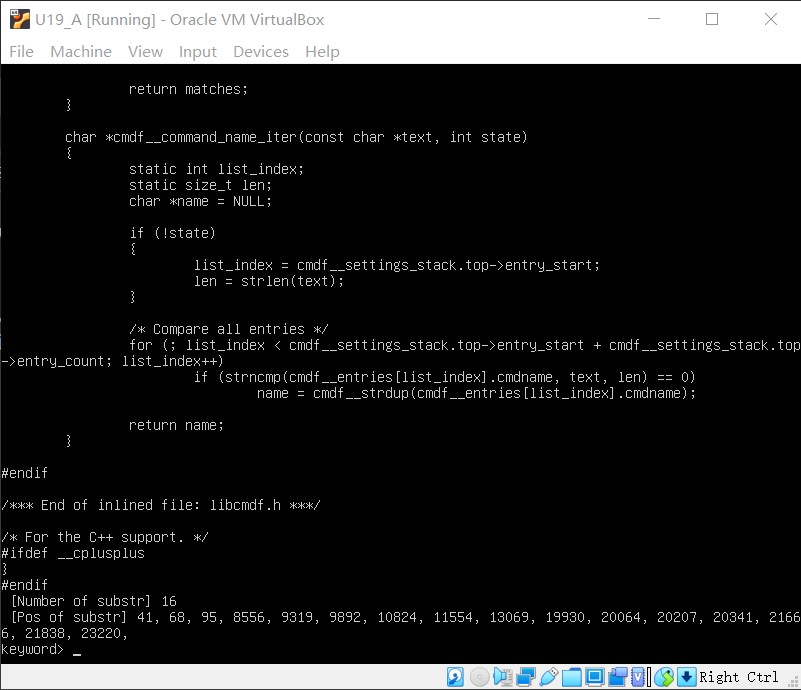
\includegraphics[width=0.6\linewidth]{image/kmp_05.jpg}
    \caption{Use \lstinline{a test.c} to append text to a file.}
\end{figure}
The results show that the operation is successful.



\section{About the string search algorithm}

\subsection{Naive string search}

The most common case of string searching involves finding one very short string(such as a word) in a long string (such as a file), and . In this situation, a simple but efficient way is to check the first char in the long string with the short string, and if they match, check next in both string. If they do not match, then start with next char in the long string. The pseudocode for the Naive string search algorithm is shown below.
\begin{algorithm}[H]
    \caption{Naive string search $(s1,s2)$}
    \label{alg1}
    \begin{algorithmic}
        \REQUIRE $len(s1) \leq len(s2) $
        \ENSURE if $s1$ in $s2$, return \textbf{TRUE}, else return \textbf{FALSE}
        \STATE Initialization: $p1 = 0$, $p2 = 0$
        \WHILE{$p2 < len(s2) - len(p1)$}
        \WHILE{$p1 < len(s1)$ and $s1[p1] = s2[p2+p1]$}
        \STATE $p1$++
        \IF{$p1 = len(s1)$}
        \STATE return \textbf{TRUE}
        \ENDIF
        \ENDWHILE
        \STATE $p1 = 0$, $p2$++
        \ENDWHILE
        \STATE return \textbf{FALSE}
    \end{algorithmic}
\end{algorithm}

The computational complexity of such algorithm is $O(mn)$ (worst cases like s1=aaa, s2=aaaaaaaaab), where $m$ is the length of s1, and $n$ is the length of s2. If s1 is not long, this method is fast enough. However, in some special situation, searching may involve finding a relatively long string (like a line of code) in a VERY long string (a code repo with millions lines of code).

\subsection{Finite-state-automaton-based method}
To avoid backtracking in the case like (s1=aaa, s2=aaaaaaaaab), we can construct a deterministic finite automaton (DFA) that recognizes stored search string. These are expensive to construct—they are usually created using the powerset construction—but are very quick to use. One example of DFA based algorithms is the \textbf{AC automaton}. Since this approach is widely used to search for arbitrary regular expressions, the author will not explain it in detail.

\subsection{Prefix function method}

The main trick of KMP algorithm is the Prefix function. The Prefix function is defined as the following:

You are given a string $s$ of length $n$. The \textbf{prefix function} for this string is defined as an array $\pi$ of length $n$, where $\pi[i]$ is the length of the longest proper prefix of the substring $s[0 \dots i]$ which is also a suffix of this substring. A proper prefix of a string is a prefix that is not equal to the string itself. By definition, $\pi[0] = 0$.

Mathematically the definition of the prefix function can be written as follows:

$$\pi[i] = \max_ {k = 0 \dots i} \\{k : s[0 \dots k-1] = s[i-(k-1) \dots i] \\}$$

For example, prefix function of string "abcabcd" is $[0, 0, 0, 1, 2, 3, 0]$, and prefix function of string "aabaaab" is $[0, 1, 0, 1, 2, 2, 3]$.

A trivial algorithm to compute a prefix function of a string is a brute-force method according to the definition. The computational complexity is $O(n^3)$, which is undesirable.

In 1977, an algorithm was proposed by Knuth and Pratt and independently which involves optimizations to the trivial algorithm.

The first important observation is, that the values of the prefix function can only increase by at most one. If not so, we can remove the last char at $i+1$ and have $\pi[i + 1] - 1 > \pi[i]$, indicating a better $\pi[i]$, which contradicts with the definition of the prefix function.

Thus when moving to the next position, the value of the prefix function can either increase by one, stay the same, or decrease by some amount. Together with all the information computed in the previous steps, we can compute the value of the prefix function $\pi$ for $i + 1$.

If $s[i+1] = s[\pi[i]]$, then we can say with certainty that $\pi[i+1] = \pi[i] + 1$, since we already know that the suffix at position $i$ of length $\pi[i]$ is equal to the prefix of length $\pi[i]$.

If this is not the case, $s[i+1] \neq s[\pi[i]]$, then we need to try a shorter string.
In order to speed things up, we would like to immediately move to the longest length $j \le \pi[i]$, such that the prefix property in the position $i$ holds, i.e. $s[0 \dots j-1] = s[i-j+1 \dots i]$.

If we find such a length $j$, then we again only need to compare the characters $s[i+1]$ and $s[j]$.If they are equal, then we can assign $\pi[i+1] = j + 1$.Otherwise we will need to find the largest value smaller than $j$, for which the prefix property holds, and so on.

The only question left is how do we effectively find the lengths for $j$.

\textbf{The MAGIC} happens here: this has to be the value of $\pi[j-1]$. According to the definition of $\pi[j-1]$, we have:
$$\overbrace{\underbrace{s_0 ~ s_1}\_k ~ s_2 ~ s_3}^j ~ \dots ~ \overbrace{s_{i-3} ~ s_{i-2} ~ \underbrace{s_{i-1} ~ s_{i}}\_k}^j ~s_{i+1}$$
And the $\pi[j-1]$ is already calculated.

The full algorithm to compute the prefix function is\uct{github:prefix}:
\begin{enumerate}
    \item We compute the prefix values $\pi[i]$ in a loop by iterating from $i = 1$ to $i = n-1$ ($\pi[0]$ just gets assigned with $0$).
    \item To calculate the current value $\pi[i]$ we set the variable $j$ denoting the length of the best suffix for $i-1$. Initially $j = \pi[i-1]$.
    \item Test if the suffix of length $j+1$ is also a prefix by comparing $s[j]$ and $s[i]$. If they are equal then we assign $\pi[i] = j + 1$, otherwise we reduce $j$ to $\pi[j-1]$ and repeat this step.
    \item If we have reached the length $j = 0$ and still don't have a match, then we assign $\pi[i] = 0$ and go to the next index $i + 1$.
\end{enumerate}
This is an $O(n)$ algorithm, which is desirable for most situations.

Then all we need to do is to put $s_0$ before $s_1$ and add a special char to separate them. We then calculate the prefix function of the new string, and count how many times the $len(s_0)$ appears in the prefix function array. The count is the number of substring in the text.

\section{Notes on the source code}

Detailed implementation of the KMP algorithm follows the textbooks used in this course. Most of the code in \lstinline{main.cpp} is for processing the user's input, which is not so interesting. The most important piece of code lies here:

\begin{lstlisting}[language = C++]
vector<int> prefixFunction(string s)
{
    int n = (int)s.length();
    vector<int> pi(n);
    for (int i = 1; i < n; i++)
    {
        int j = pi[i - 1];
        while (j > 0 && s[i] != s[j])
            j = pi[j - 1];
        if (s[i] == s[j])
            j++;
        pi[i] = j;
    }
    return pi;
};
\end{lstlisting}

This short and elegant code calculates the prefix function of $s_0+s_1$, and a simple count of the vector can do the rest of work.

\section{Discussion}

Other string search methods, like the AC automaton, can achieve the same efficiency, but none of them can have such elegant implementation. Also, the math behind the KMP algorithm is simple, but a student like the author can be surprised when the magic $j \gets \pi[j-1]$ was put forward.

\bibliography{references}
\end{document}
